\chapter{Results}
\label{chap:results}
% Figure macros for Chapter 4 (Results).

\newcommand{\figResultsOverview}{%
\begin{figure}[!htbp]
\centering
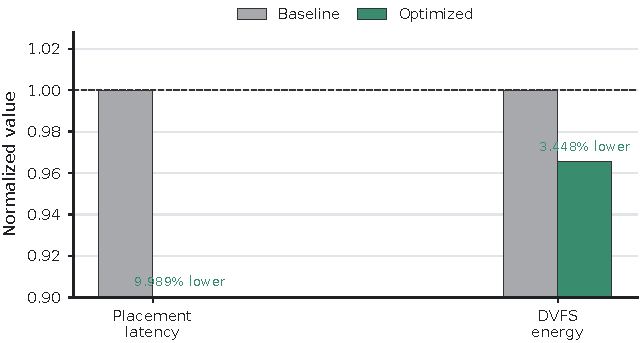
\includegraphics[width=0.86\linewidth]{figures/results_overview.pdf}
\caption{Overview of the two main evaluation outcomes. Placement reports normalized latency relative to HEFT, while DVFS reports normalized energy relative to no-DVFS execution. The y-axis is truncated to make the normalized differences visible.}
\label{fig:results-overview}
\end{figure}%
}

\newcommand{\figBenchmarkCopyVolume}{%
\begin{figure}[!htbp]
\centering
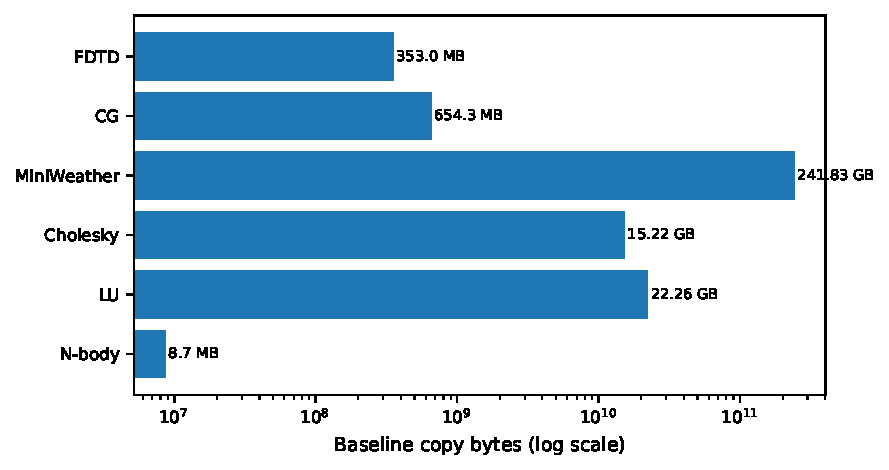
\includegraphics[width=0.86\linewidth]{figures/benchmark_copy_volume.pdf}
\caption{Baseline copy volume for the benchmark suite. The log-scale x-axis separates absolute copy traffic from residual-placement opportunity: MiniWeather has large baseline copy volume, but the placement measurements show little reducible copy traffic under the residual policy.}
\label{fig:results-benchmark-copy-volume}
\end{figure}%
}

\newcommand{\figPlacementDeltas}{%
\begin{figure}[!htbp]
\centering
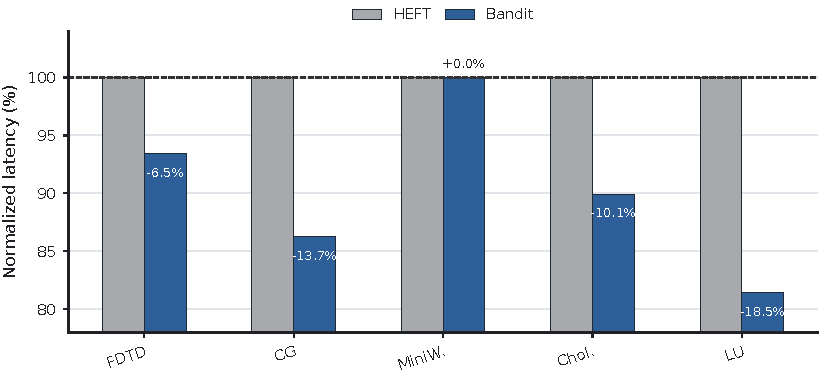
\includegraphics[width=0.94\linewidth]{figures/placement_deltas.pdf}
\caption{Normalized placement latency relative to HEFT. HEFT is fixed at \(100\%\) for each benchmark, and the Bandit bars show the corresponding normalized latency reduction.}
\label{fig:results-placement-deltas}
\end{figure}%
}

\newcommand{\figCopyLatencyScatter}{%
\begin{figure}[!htbp]
\centering
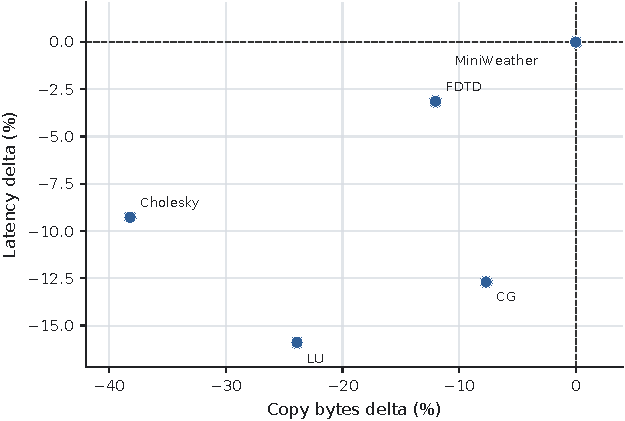
\includegraphics[width=0.78\linewidth]{figures/copy_latency_scatter.pdf}
\caption{Relationship between copy-byte reduction and placement latency reduction. CG uses copy counters from the placement measurements because the locality diagnostic set does not include a CG deviation-rate row.}
\label{fig:results-copy-latency}
\end{figure}%
}

\newcommand{\figDeviationLatencyScatter}{%
\begin{figure}[!htbp]
\centering
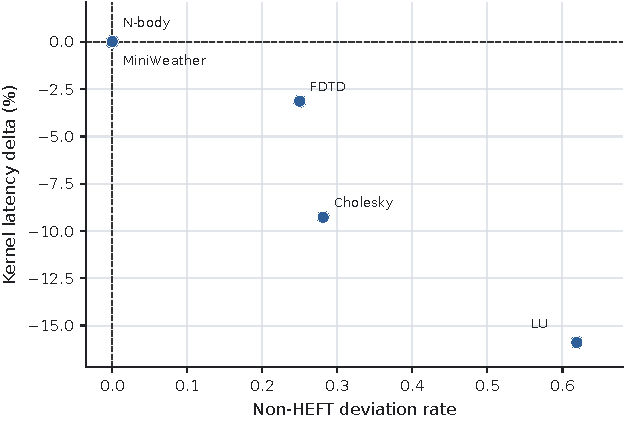
\includegraphics[width=0.78\linewidth]{figures/deviation_latency_scatter.pdf}
\caption{Scheduler deviation rate and placement latency improvement in the locality diagnostic measurements. Deviation frequency is explanatory, not a direct linear predictor of speedup. CG is omitted because the diagnostic set does not contain its deviation-rate row.}
\label{fig:results-deviation-latency}
\end{figure}%
}

\newcommand{\figDvfsDeltas}{%
\begin{figure}[!htbp]
\centering
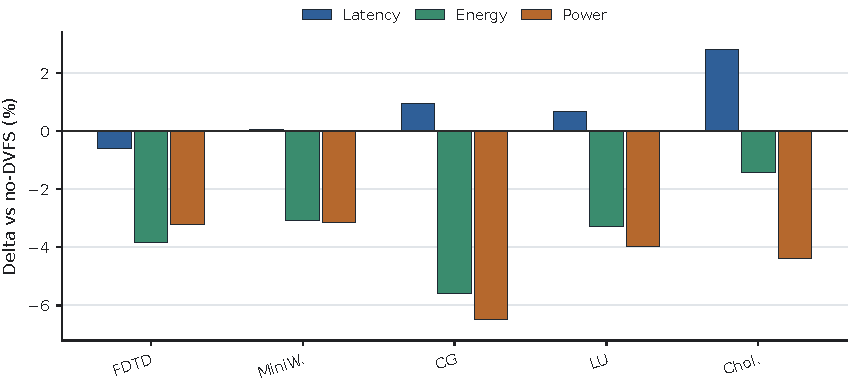
\includegraphics[width=0.94\linewidth]{figures/dvfs_deltas.pdf}
\caption{Per-benchmark DVFS latency, energy, and power deltas relative to no-DVFS execution. The figure reports power together with energy and latency because lower power alone is not sufficient if runtime increases too much.}
\label{fig:results-dvfs-deltas}
\end{figure}%
}

\newcommand{\figDvfsTradeoff}{%
\begin{figure}[!htbp]
\centering
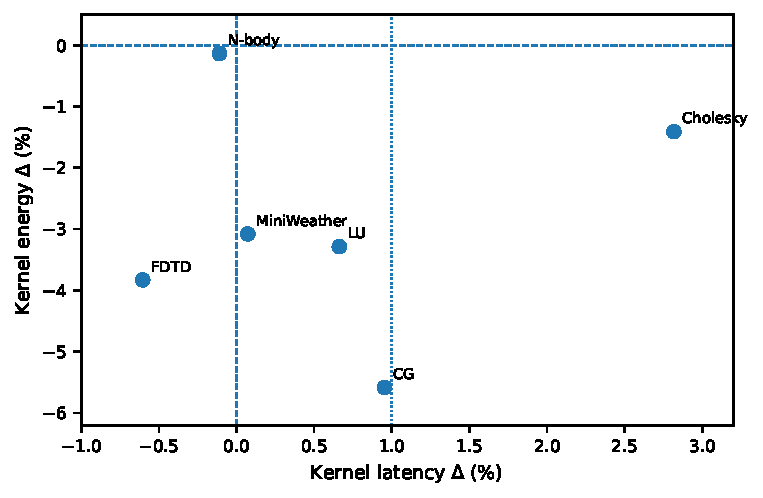
\includegraphics[width=0.78\linewidth]{figures/dvfs_tradeoff.pdf}
\caption{Energy--latency trade-off of WinDVFS. The dotted vertical line marks a 1\% latency-overhead reference. Points below the horizontal axis reduce energy; points to the left of the vertical axis also reduce latency.}
\label{fig:results-dvfs-tradeoff}
\end{figure}%
}

\newcommand{\figDvfsEdpRatios}{%
\begin{figure}[!htbp]
\centering
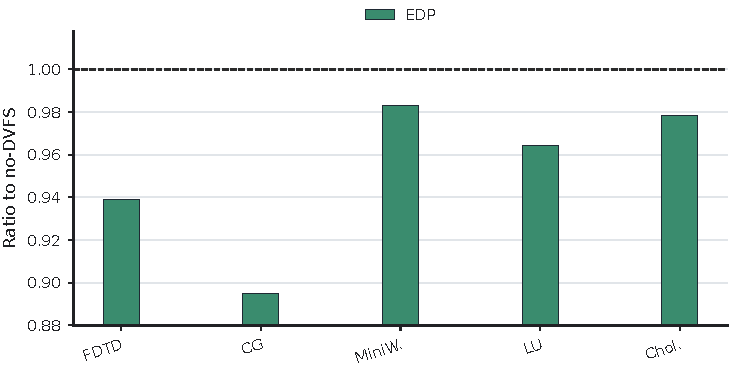
\includegraphics[width=0.94\linewidth]{figures/dvfs_edp_ratios.pdf}
\caption{DVFS EDP ratios relative to no-DVFS execution. Values below the dashed 1.0 line indicate improvement after accounting for runtime.}
\label{fig:results-dvfs-edp-ratios}
\end{figure}%
}

\newcommand{\figMidEnergyScatter}{%
\begin{figure}[!htbp]
\centering
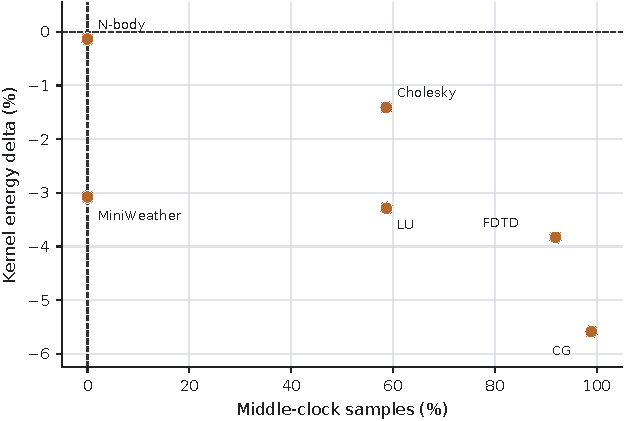
\includegraphics[width=0.78\linewidth]{figures/mid_energy_scatter.pdf}
\caption{Middle-clock sample share and energy reduction. MiniWeather is an exception to a simple residency-based explanation because its measured energy decreases despite zero middle-clock samples.}
\label{fig:results-mid-energy}
\end{figure}%
}

\newcommand{\figDvfsCommitShare}{%
\begin{figure}[!htbp]
\centering
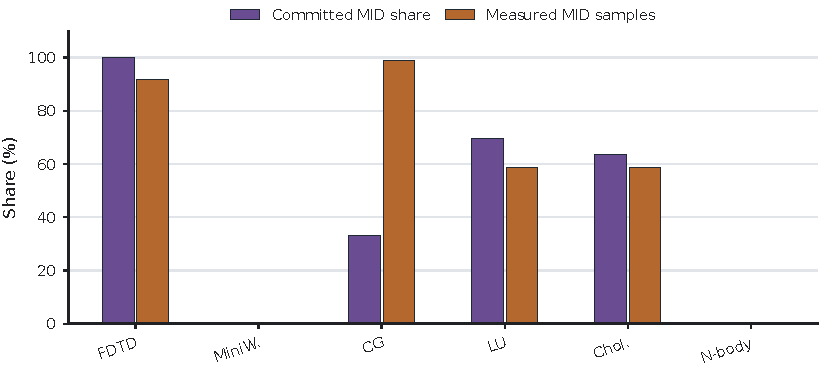
\includegraphics[width=0.94\linewidth]{figures/dvfs_commit_share.pdf}
\caption{Controller-reported committed MID share compared with measured middle-clock sample share. The two quantities are related but not identical because clock samples are collected at NVML sampling timestamps, whereas committed share is reported by the controller.}
\label{fig:results-dvfs-commit-share}
\end{figure}%
}

\newcommand{\figDvfsGuardrailEvents}{%
\begin{figure}[!htbp]
\centering
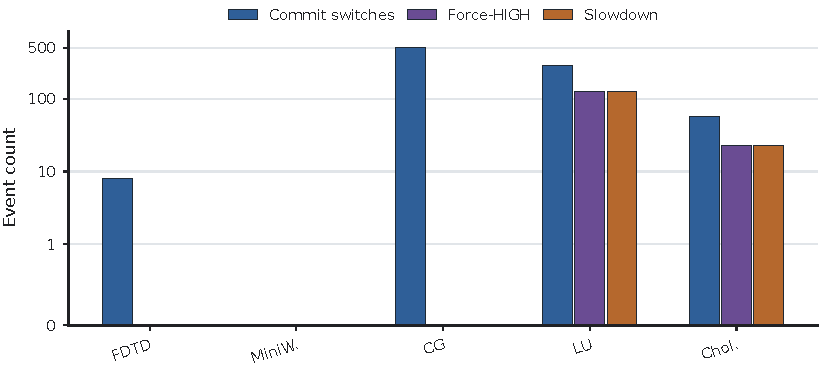
\includegraphics[width=0.94\linewidth]{figures/dvfs_guardrail_events.pdf}
\caption{DVFS commit-switch and guardrail-event counts for the final DVFS measurements. The y-axis uses a symmetric log scale so that zero and small-count workloads can be shown together with CG and LU decomposition.}
\label{fig:results-dvfs-guardrail-events}
\end{figure}%
}

\newcommand{\figOverheadSnapshot}{%
\begin{figure}[!htbp]
\centering
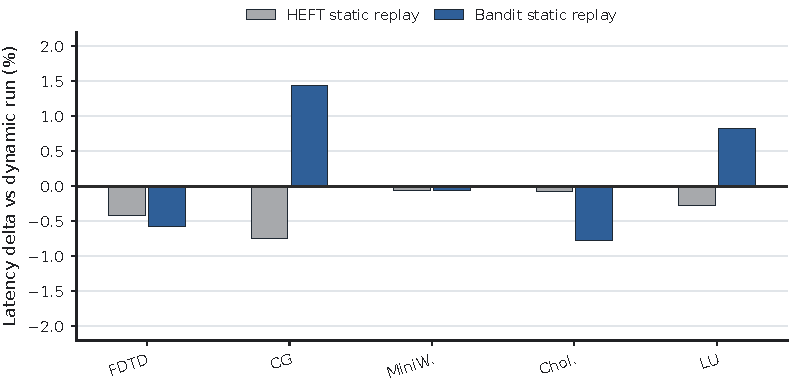
\includegraphics[width=0.86\linewidth]{figures/overhead_snapshot.pdf}
\caption{Diagnostic overhead snapshot for compact placement logging and the WinDVFS diagnostic row. These rows are diagnostic stress checks and are not used to compute the primary placement or DVFS results.}
\label{fig:results-overhead-snapshot}
\end{figure}%
}


This chapter evaluates the CUDASTF runtime scheduler on a single-node
multi-GPU platform. It first defines the experimental platform and metrics,
then states the evaluation plan, reports the headline results visually and
numerically, and finally uses data movement, clock, and power evidence to
explain the main placement and DVFS outcomes.

\section{Experimental Setup}
\label{sec:results-setup}

All experiments run on a single Slurm-managed node with eight NVIDIA L4 GPUs.
The application-visible GPU set contains all eight GPUs, and power sampling is
also performed across the same eight devices. This keeps the placement and
energy measurements aligned: the scheduler can place work on any of the eight
GPUs, and the energy measurement covers the same device set.

Table~\ref{tab:results-platform} summarizes the hardware and software
configuration. The benchmark executable and the power-sampling process run
inside the same Apptainer environment so that compiler, CUDA runtime, and
library versions remain fixed across the evaluation.

\begin{table}[H]
\centering
\small
\begin{tabular}{@{}ll@{}}
\toprule
Component & Configuration \\
\midrule
Node manager & Slurm-managed single node \\
GPUs & 8 NVIDIA L4 GPUs \\
Application-visible GPUs & 0--7 \\
GPU power limit & 72 W per GPU \\
Container runtime & Apptainer \\
Build type & Release \\
CUDA version & CUDA 12.4.1 \\
NVCC version & 12.4.131 \\
GCC version & 11.4 \\
CUDA architecture & sm\_89 \\
High SM clock & approximately 2040 MHz \\
Middle SM clock target & 1875 MHz \\
Memory clock & 6251 MHz \\
Power sampling & NVML samples across all eight visible GPUs \\
\bottomrule
\end{tabular}
\caption{Hardware and software configuration used in the evaluation.}
\label{tab:results-platform}
\end{table}

The NVIDIA L4 platform exposes application-clock control through NVML. The
evaluated DVFS policy changes the SM clock level but keeps the memory clock at
6251 MHz. The results therefore evaluate a conservative core-frequency control
path rather than a combined core-and-memory frequency policy.

Table~\ref{tab:results-benchmark-characteristics} summarizes the benchmark
inputs and observed task-graph scale. The opportunity label refers to the
expected opportunity for residual placement to find useful non-HEFT
alternatives. It is not simply the absolute amount of baseline copy traffic. A
benchmark may have large copy volume but little residual-placement opportunity
if the copy pattern is structurally fixed or if the HEFT baseline already
preserves the relevant locality. The suite intentionally includes both
copy-sensitive task graphs and near-neutral task graphs so that the evaluation
can test whether the scheduler improves favorable cases without forcing
changes where there is little opportunity.

\begin{table}[H]
\centering
\small
\resizebox{\linewidth}{!}{%
\begin{tabular}{@{}llrrl@{}}
\toprule
Benchmark & Problem size / input & Tasks & Baseline copy bytes & Expected residual-placement opportunity \\
\midrule
FDTD & 3840, 288, 288, 288 & 491712 & 353009664 & medium \\
CG & 16777216, 64, 4, 1e-10 & 34 & 654311738 & medium \\
MiniWeather & 1600, 2048, 1536 & 57600 & 241833733942 & low \\
Cholesky & 49152, 2048 & 2600 & 15221178776 & high \\
LU decomposition & 25088, 256 & 318549 & 22258961026 & high \\
Blocked N-body & 49152, 512, 14 & 131712 & 8659968 & low \\
\bottomrule
\end{tabular}%
}
\caption{Benchmark characteristics from the placement-run raw data.}
\label{tab:results-benchmark-characteristics}
\end{table}

\section{Metrics and Measurement Methodology}
\label{sec:results-metrics}

\textbf{Kernel latency:}
Kernel latency is the primary performance metric. It measures the benchmark's
GPU kernel-window duration and is used for both placement and DVFS performance
comparisons. This metric excludes unrelated process startup, final output, and
host-side bookkeeping, so it focuses on the execution interval affected by the
runtime scheduler.

\textbf{Kernel energy:}
Kernel energy is the primary energy metric for DVFS. At each NVML sampling
timestamp, the result scripts record power readings for the eight visible GPUs.
Kernel energy is computed by trapezoidal integration over the kernel-window
samples. The final-source rows have an observed sampling interval of
approximately 100 ms, so the estimate is limited by NVML sampling resolution,
especially when clock transitions are short relative to the sampling period.

\textbf{Kernel power:}
Kernel power is the average NVML power over the kernel window. It is reported
to explain energy changes, not as the headline objective by itself. A lower
average power only improves energy if the corresponding runtime increase is
small enough.

\textbf{Whole-process energy:}
Whole-process energy is measured as an auxiliary diagnostic but is not used for
the main claims. It includes startup, initialization, host-side work, and final
output handling, whereas both the placement scheduler and the DVFS controller
act on the GPU kernel execution window.

\textbf{Speedup and geometric means:}
Placement speedup is computed as HEFT kernel latency divided by scheduler
kernel latency. Suite-level summaries use geometric means so that each
benchmark contributes multiplicatively rather than allowing one large absolute
runtime to dominate the aggregate.

\textbf{Relative deltas:}
Relative deltas are computed against the baseline named in the corresponding
section. For placement, the baseline is HEFT with DVFS disabled. For DVFS, the
baseline is no-DVFS execution under the same placement layer. Negative deltas
in latency, energy, power, and copy traffic indicate reductions relative to
that baseline.

\textbf{EDP and ED\(^2\)P:}
Energy--delay product is reported for DVFS as \(E \times T\), and ED\(^2\)P as
\(E \times T^2\). These ratios show whether energy savings still hold after
accounting for runtime changes, especially for latency-sensitive workloads.

\textbf{Data-movement and DVFS evidence:}
Copy-byte reduction, copy-time reduction, and non-HEFT deviation rate are used
as placement locality evidence. Average SM clock, middle-clock sample share,
and commit or guardrail counters are used as DVFS evidence. These supporting
measurements explain the observed latency and energy changes, but the headline
claims are based on kernel latency and kernel energy.

\textbf{Evidence roles:}
The measurements in this chapter have different evidential roles. Placement
performance is the headline latency result; locality rows are diagnostic
attribution; DVFS rows are final energy--performance measurements under the
evaluated configuration; and the overhead table is a diagnostic stress check
rather than a production-overhead estimate.

\section{Evaluation Plan}
\label{sec:results-plan}

The evaluation separates placement from frequency control. The placement
experiments compare HEFT with the bandit scheduler while DVFS is disabled. The
DVFS experiments hold the placement layer fixed and compare WinDVFS against a
no-DVFS baseline using kernel energy as the main metric. This isolation is
important because placement changes where work runs, whereas DVFS changes the
frequency at which the selected GPUs execute that work.

Table~\ref{tab:results-eval-configs} makes this separation explicit. The
placement-only experiments answer whether the residual scheduler improves
latency. The data-movement diagnostic experiments then check whether those
latency changes are consistent with locality. The DVFS experiments are
reported separately, with no-DVFS execution as the energy baseline.

\begin{table}[H]
\centering
\small
\resizebox{\linewidth}{!}{%
\begin{tabular}{@{}llll@{}}
\toprule
Experiment & Placement policy & DVFS policy & Main metric \\
\midrule
Placement-only & HEFT vs bandit scheduler & disabled & kernel latency \\
Data-movement diagnostic & HEFT vs bandit scheduler & disabled & copy bytes and copy time \\
DVFS final & fixed placement layer & no-DVFS vs WinDVFS & kernel energy \\
Clock and power evidence & fixed placement layer & no-DVFS vs WinDVFS & SM clock and kernel power \\
Overhead diagnostic & selected scheduler/control rows & mixed diagnostic rows & kernel latency and energy \\
\bottomrule
\end{tabular}%
}
\caption{Evaluation configuration matrix.}
\label{tab:results-eval-configs}
\end{table}

The results are then presented in the same evidence order. The placement
section reports the latency and energy deltas relative to HEFT. The
data-movement section checks whether those deltas align with copy-volume
reductions. The DVFS section reports the energy result relative to no-DVFS
execution, while the clock, power, and guardrail section explains why the
energy reductions appear on some workloads but not on all of them. The chapter
ends with an overhead diagnostic and an explicit statement of the boundaries of
the claims, rather than mixing diagnostic details into the main result tables.

\figResultsOverview

\section{Placement Performance}
\label{sec:results-placement-performance}

Figure~\ref{fig:results-placement-deltas} visualizes the placement-only
latency and kernel-energy deltas for each benchmark, while
Table~\ref{tab:results-placement-main} reports the exact numerical values. The
figure separates the benchmark suite into three behaviors: strong
placement-benefit workloads, represented by CG, Cholesky, and LU
decomposition; a modest positive case, represented by FDTD; and near-neutral
workloads, represented by MiniWeather and Blocked N-body. This separation is
important because the proposed scheduler is expected to exploit locality only
when the task graph exposes useful placement alternatives.

\figPlacementDeltas

\begin{table}[H]
\centering
\small
\begin{tabular}{@{}lrrr@{}}
\toprule
Benchmark & Speedup & Kernel latency \(\Delta\) & Kernel energy \(\Delta\) \\
\midrule
FDTD & \(1.0135\times\) & \(-1.333\%\) & \(-0.597\%\) \\
CG & \(1.1454\times\) & \(-12.693\%\) & \(-12.316\%\) \\
MiniWeather & \(0.9998\times\) & \(+0.019\%\) & \(-0.062\%\) \\
Cholesky & \(1.0945\times\) & \(-8.638\%\) & \(-2.441\%\) \\
LU decomposition & \(1.2276\times\) & \(-18.539\%\) & \(-17.872\%\) \\
Blocked N-body & \(1.0005\times\) & \(-0.052\%\) & \(-0.580\%\) \\
\bottomrule
\end{tabular}
\caption{Placement-only results relative to HEFT. DVFS is disabled.}
\label{tab:results-placement-main}
\end{table}

The six-benchmark geometric-mean speedup is \(1.076965\times\), equivalent to
a \(7.146\%\) normalized latency reduction. The distribution of the result is
more important than a single suite number. LU decomposition has the largest
gain, followed by CG and Cholesky. These three workloads dominate the
placement benefit because their task graphs expose useful alternatives to the
HEFT placement. FDTD is a modest positive case. MiniWeather and Blocked
N-body are effectively unchanged, showing that the scheduler does not need to
move work aggressively when there is little locality benefit.

The geometric mean should therefore be interpreted as a suite-level summary,
not as evidence that every benchmark benefits equally. FDTD is used only as a
weak positive placement case because its latency improvement is modest. The
stronger placement evidence comes from CG, Cholesky, and LU decomposition,
where the effect sizes are substantially larger.

The energy column is included to show that the placement-only runs do not
hide a performance--energy reversal. CG and LU decomposition reduce both
latency and kernel energy, while the neutral workloads remain near the
baseline. The placement claim itself, however, is based on latency and
locality evidence rather than on DVFS-style energy control.

\section{Placement Locality Evidence}
\label{sec:results-locality-attribution}

The copy-traffic measurements are used as explanatory evidence rather than as
a separate performance objective. A placement improvement is more credible when
reduced latency coincides with reduced copy volume or copy time, because this
indicates that the scheduler is exploiting locality rather than only benefiting
from run-to-run noise.

Table~\ref{tab:results-locality-attribution} connects the placement result to
copy traffic. Most rows come from instrumented locality diagnostic runs, so
their latency deltas are not used to compute the headline speedup reported in
Table~\ref{tab:results-placement-main}. They are used to check whether the
direction of the placement effect is consistent with reduced copy traffic. CG
was not included in the locality diagnostic run set; its row therefore uses
the copy counters from the placement batch and omits the diagnostic deviation
rate.

\begin{table}[H]
\centering
\small
\resizebox{\linewidth}{!}{%
\begin{tabular}{@{}lrrrrcl@{}}
\toprule
Benchmark & Kernel latency \(\Delta\) & Speedup & Copy bytes \(\Delta\) & Copy time \(\Delta\) & Deviation rate & Source \\
\midrule
FDTD & \(-3.135\%\) & \(1.0324\times\) & \(-12.030\%\) & \(-12.025\%\) & 0.249902 & Diagnostic \\
CG & \(-12.693\%\) & \(1.1454\times\) & \(-7.692\%\) & \(-7.688\%\) & -- & Placement batch \\
MiniWeather & \(-0.0066\%\) & \(1.0001\times\) & \(0.000\%\) & \(0.000\%\) & 0.000000 & Diagnostic \\
Cholesky & \(-9.269\%\) & \(1.1022\times\) & \(-38.220\%\) & \(-38.220\%\) & 0.281154 & Diagnostic \\
LU decomposition & \(-15.891\%\) & \(1.1889\times\) & \(-23.905\%\) & \(-23.905\%\) & 0.619305 & Diagnostic \\
Blocked N-body & \(+0.019\%\) & \(0.9998\times\) & \(0.000\%\) & \(0.000\%\) & 0.000000 & Diagnostic \\
\bottomrule
\end{tabular}%
}
\caption{Data-movement evidence for the placement result. Negative latency, copy-byte, and copy-time deltas are reductions relative to HEFT. CG uses placement-run copy counters; the other rows are locality diagnostic rows.}
\label{tab:results-locality-attribution}
\end{table}

\figCopyLatencyScatter

\figDeviationLatencyScatter

The locality data separates the benchmarks into two groups. For LU
decomposition, Cholesky, and FDTD, the diagnostic rows show that latency
improvements coincide with lower copy volume and lower measured copy time. CG
shows the same direction in the placement-batch copy counters, but because it
lacks a diagnostic deviation-rate row, it is treated as placement-performance
evidence rather than as one of the cleanest locality-attribution cases.
Figure~\ref{fig:results-copy-latency} shows this relationship directly. The
zero-copy-reduction workloads cluster near zero latency change, while the
copy-reducing workloads move into the latency-improvement region.

Figure~\ref{fig:results-deviation-latency} shows that the residual scheduler is
selective, but the deviation rate should be interpreted as the frequency of
non-HEFT decisions rather than as a direct predictor of speedup. The benefit
depends on whether the deviations remove costly copies. LU decomposition
deviates most often and has the strongest locality-driven speedup, while
Cholesky obtains a large copy reduction from a smaller deviation rate. FDTD is
the weaker copy-saving case, but still follows the same direction.

MiniWeather and Blocked N-body provide the contrast case. Their deviation
rates are zero, copy traffic is unchanged, and latency remains effectively at
the HEFT baseline. This contrast supports the interpretation that the residual
policy is selective: it changes placements when copy-saving opportunities are
visible and otherwise collapses back to HEFT-like behavior.

\section{DVFS Energy--Performance Trade-off}
\label{sec:results-dvfs-energy}

DVFS is evaluated as an energy--performance trade-off rather than as a pure
power-reduction objective. Lower average power does not necessarily imply lower
energy if runtime increases too much. Unlike the placement headline, the DVFS
result is interpreted as a final-configuration energy--performance measurement
rather than as a repeated-run statistical comparison. The analysis therefore
emphasizes multi-percent energy changes and treats sub-percent changes as
near-neutral unless they are supported by the broader power, clock, or
trade-off evidence. Figure~\ref{fig:results-dvfs-deltas} therefore reports
latency, energy, and power together, and Table~\ref{tab:results-dvfs-energy}
gives the exact values.

\figDvfsDeltas

\begin{table}[H]
\centering
\small
\begin{tabular}{@{}lrrr@{}}
\toprule
Benchmark & Kernel latency \(\Delta\) & Kernel energy \(\Delta\) & Kernel power \(\Delta\) \\
\midrule
FDTD & \(-0.604\%\) & \(-3.829\%\) & \(-3.230\%\) \\
MiniWeather & \(+0.073\%\) & \(-3.079\%\) & \(-3.150\%\) \\
CG & \(+0.953\%\) & \(-5.587\%\) & \(-6.478\%\) \\
LU decomposition & \(+0.662\%\) & \(-3.287\%\) & \(-3.968\%\) \\
Cholesky & \(+2.817\%\) & \(-1.411\%\) & \(-4.389\%\) \\
Blocked N-body & \(-0.110\%\) & \(-0.137\%\) & \(-0.023\%\) \\
\bottomrule
\end{tabular}
\caption{Final WinDVFS result relative to no-DVFS execution. Energy and power are kernel-window NVML metrics.}
\label{tab:results-dvfs-energy}
\end{table}

Across the six benchmarks, the geometric-mean kernel-energy ratio is
0.970962, corresponding to \(2.904\%\) lower normalized kernel energy. The
geometric-mean latency ratio is 1.006259, corresponding to a \(0.626\%\)
latency overhead. This is the main DVFS result: guarded window-level frequency
control reduces kernel energy on this benchmark set while keeping aggregate
latency cost below one percent.

\figDvfsTradeoff

Figure~\ref{fig:results-dvfs-tradeoff} shows why the aggregate result needs to
be read as a trade-off. FDTD is close to the ideal lower-latency and
lower-energy region. MiniWeather, CG, and LU decomposition reduce energy with
less than one percent latency overhead. Cholesky is the main less-favorable
case: its average kernel power decreases by \(4.389\%\), but the \(2.817\%\)
latency increase offsets much of the power saving, leaving a \(1.411\%\)
kernel-energy reduction. Blocked N-body stays close to the origin and is
therefore treated as near-neutral.

\begin{table}[H]
\centering
\small
\begin{tabular}{@{}lrr@{}}
\toprule
Benchmark & EDP ratio & ED\(^2\)P ratio \\
\midrule
FDTD & 0.955902 & 0.950133 \\
MiniWeather & 0.969913 & 0.970618 \\
CG & 0.953132 & 0.962218 \\
LU decomposition & 0.973536 & 0.979985 \\
Cholesky & 1.013666 & 1.042219 \\
Blocked N-body & 0.997531 & 0.996431 \\
\midrule
Geometric mean & 0.977040 & 0.983155 \\
\bottomrule
\end{tabular}
\caption{DVFS energy--delay ratios computed from the kernel-energy and kernel-latency ratios in Table~\ref{tab:results-dvfs-energy}. Values below 1.0 indicate improvement.}
\label{tab:results-dvfs-edp}
\end{table}

The EDP and ED\(^2\)P ratios reinforce the same interpretation. The suite-level
energy--delay products improve, but Cholesky crosses above 1.0 because its
latency overhead is large enough to dominate the modest energy saving. This
marks Cholesky as a latency-sensitive trade-off case rather than a headline
DVFS win.

\section{Clock, Power, and Guardrail Evidence}
\label{sec:results-dvfs-clock-guardrail}

Table~\ref{tab:results-dvfs-clock} reports the clock and power data behind the
DVFS result. The larger energy reductions coincide with lower average kernel
power and visible exposure to the middle SM clock. The neutral Blocked N-body
row shows almost no movement in clock or power.

\begin{table}[H]
\centering
\small
\resizebox{\linewidth}{!}{%
\begin{tabular}{@{}lrrrr@{}}
\toprule
Benchmark & Base SM MHz & WinDVFS SM MHz & MID samples & Kernel energy \(\Delta\) \\
\midrule
FDTD & 1931.442 & 1852.530 & 91.903\% & \(-3.829\%\) \\
MiniWeather & 2040.000 & 2028.091 & 0.000\% & \(-3.079\%\) \\
CG & 2032.581 & 1876.795 & 98.912\% & \(-5.587\%\) \\
LU decomposition & 2040.000 & 1943.170 & 58.685\% & \(-3.287\%\) \\
Cholesky & 2040.000 & 1943.222 & 58.654\% & \(-1.411\%\) \\
Blocked N-body & 2040.000 & 2040.000 & 0.000\% & \(-0.137\%\) \\
\bottomrule
\end{tabular}%
}
\caption{Clock and energy data for the WinDVFS rows. MID samples report the fraction of kernel-window samples at the middle SM clock level.}
\label{tab:results-dvfs-clock}
\end{table}

\figMidEnergyScatter

The clock data explains why the DVFS result is workload dependent. CG and FDTD
have high middle-clock exposure and clear energy reductions. LU decomposition
and Cholesky show partial middle-clock exposure; LU decomposition keeps the
latency cost small, while Cholesky exposes the expected trade-off between lower
power and longer runtime.

MiniWeather is the main exception to a simple middle-clock-residency
interpretation. Its MID-sample share is zero, but its average SM clock and
average kernel power are still slightly lower than the no-DVFS baseline. This
suggests that the measured energy reduction may be influenced by short clock
transitions, sampling granularity, or device-level power-management behavior
rather than sustained residence at the nominal middle clock. For this reason,
MiniWeather is treated as a measured energy-saving case, but not as the
strongest evidence of sustained middle-clock execution.

Table~\ref{tab:results-dvfs-guardrail} reports the realized commit and
guardrail counters for the final-source DVFS rows. These counters are not
additional performance metrics; they show whether the clock outcome in
Table~\ref{tab:results-dvfs-clock} came from sustained MID commits, no committed
clock change, or guardrail recovery to higher clocks.

\begin{table}[H]
\centering
\small
\resizebox{\linewidth}{!}{%
\begin{tabular}{@{}lrrrrr@{}}
\toprule
Benchmark & Effective MID share & MID samples & Commit switches & Force-HIGH events & Slowdown events \\
\midrule
FDTD & 1.000 & 91.903\% & 8 & 0 & 0 \\
MiniWeather & 0.000 & 0.000\% & 0 & 0 & 0 \\
CG & 0.333 & 98.912\% & 512 & 0 & 0 \\
LU decomposition & 0.697 & 58.685\% & 290 & 127 & 127 \\
Cholesky & 0.637 & 58.654\% & 57 & 23 & 23 \\
Blocked N-body & 0.000 & 0.000\% & 0 & 0 & 0 \\
\bottomrule
\end{tabular}%
}
\caption{DVFS commit and guardrail counters for the final-source rows. Effective MID share is the committed-time share reported by the controller; MID samples are measured from kernel-window clock samples.}
\label{tab:results-dvfs-guardrail}
\end{table}

The guardrail counters refine the clock interpretation. FDTD and CG have high
measured middle-clock exposure without slowdown recovery events. LU
decomposition and Cholesky show partial MID exposure together with force-HIGH
and slowdown events, so their rows are better read as guarded trade-offs than
as unconstrained down-clocking. MiniWeather and Blocked N-body have no committed
MID share in these final-source rows.

Blocked N-body serves as a near-neutral control case. In the placement
experiment, its copy-byte reduction and deviation rate are both zero, and its
latency remains essentially unchanged. In the DVFS experiment, its SM clock
remains at 2040 MHz and its kernel power changes by only \(-0.023\%\). These
observations suggest that both the placement layer and the DVFS layer avoid
unnecessary intervention when the workload does not expose useful locality or
frequency-scaling opportunity.

\section{Diagnostic Overheads and Claim Boundaries}
\label{sec:results-overhead}

Table~\ref{tab:results-overhead} reports the compact logging/control overhead
snapshot. It should be read as a diagnostic stress check rather than as a
production-overhead estimate.

\begin{table}[H]
\centering
\small
\resizebox{\linewidth}{!}{%
\begin{tabular}{@{}lrrr@{}}
\toprule
Benchmark & Compact placement-log latency \(\Delta\) & WinDVFS control-row latency \(\Delta\) & WinDVFS control-row energy \(\Delta\) \\
\midrule
FDTD & \(-0.159\%\) & \(+0.953\%\) & \(-1.196\%\) \\
LU decomposition & \(+1.559\%\) & \(+9.331\%\) & \(+7.233\%\) \\
Blocked N-body & \(+0.000\%\) & \(+4.369\%\) & \(+0.722\%\) \\
\bottomrule
\end{tabular}%
}
\caption{Single-run diagnostic overhead snapshot. The compact placement-log row compares compact logging against a no-log bandit baseline. The WinDVFS control row mixes policy behavior, clock changes, and compact control logging. These rows are not production-overhead estimates and are not used to compute the headline placement or DVFS results.}
\label{tab:results-overhead}
\end{table}

The compact placement-log row isolates compact logging more directly, whereas
the WinDVFS control row combines policy behavior, frequency changes, and
compact control logging. These rows therefore do not contradict the final DVFS
validation rows; they show that detailed diagnostic control paths can become
visible in runtime and should be separated from the no-log or validation rows
used for final claims. In this snapshot, compact placement logging is close to
noise-scale for FDTD and Blocked N-body, while LU decomposition shows a visible
single-run cost.

The evaluation has four main limitations. First, all results are measured on a
single eight-GPU node, so the magnitude of the results may change with GPU
generation, interconnect topology, driver behavior, and benchmark scale.
Second, FDTD is noisier than the linear-algebra workloads and should be read as
a modest locality case rather than as the strongest placement example. Third,
NVML sampling is approximately 100 ms in the final-source rows, so very short
clock transitions may not be captured as sustained middle-clock residency.
Fourth, the DVFS conclusion is based on kernel-window energy and latency; it
does not replace a full-system power study.

\section{Results Summary}
\label{sec:results-summary}

The experimental evidence supports both layers of the proposed design. The
bandit scheduler improves geometric-mean kernel latency by \(7.146\%\) relative
to HEFT, with the largest gains appearing on copy-sensitive workloads. The
data-movement results are consistent with a locality-driven explanation of
these gains: the strongest placement cases reduce copy traffic, while the
near-neutral workloads remain close to HEFT.

WinDVFS reduces geometric-mean kernel energy by \(2.904\%\) with \(0.626\%\)
geometric-mean latency overhead. The EDP and ED\(^2\)P ratios also improve at
the suite level, but the benchmark-level trade-off matters: Cholesky shows that
lower power can be partly offset by longer runtime, while Blocked N-body stays
near the no-DVFS baseline.

The boundary of the claim is therefore explicit. The placement result is a
locality-sensitive latency improvement, not a claim that every task graph
benefits equally. The DVFS result is a kernel-window energy result on one
eight-GPU L4 node, not a full-system energy study. Within these boundaries,
this chapter shows two measured outcomes: the placement layer improves
suite-level kernel latency while preserving near-baseline behavior on
low-opportunity workloads, and the DVFS layer reduces suite-level kernel energy
while keeping the geometric-mean latency overhead below one percent.
